\documentclass[12pt, letterpaper]{../assignment}
\usepackage{graphicx}
\usepackage{courier}
\usepackage{minted}
\usepackage{amsmath}
\usepackage{polynom}
\usepackage{commath}
\usepackage{amssymb}
\usepackage{amsfonts} 
\usepackage{color}
\usepackage{cancel}
\usepackage{enumitem}
\usepackage{graphicx}
\usepackage{multirow}
\usepackage{float}
\usepackage{bm}
\usepackage{tikz}
\usetikzlibrary{shapes,arrows}
\usepackage{booktabs}
\usetikzlibrary{patterns}

% Define Theme Colors
\definecolor{light-gray}{rgb}{0.2,0.2,0.2}
\definecolor{header-blue}{rgb}{0,0,0.7}
% \definecolor{header-blue}{rgb}{0.5137,0.8353,0.9176}
\definecolor{header-blue}{rgb}{0,0.8,0.95}
\definecolor{dark-gray}{rgb}{0.1,0.1,0.1}
\pagecolor{dark-gray}
\color{white}

\usemintedstyle{monokai}
\oddsidemargin = 0pt
\exercisesheet{Module 10}{Assignment}
\student{Austin Barrilleaux}
\university{\color{header-blue}Johns Hopkins University}
\school{\color{header-blue}Whiting School of Engineering}
\courselabel{EN 535.612}
\semester{Fall 2024}
\usepackage[backend=bibtex,style=numeric,sorting=none]{biblatex}
\bibliography{reference}

\definecolor{light-gray}{rgb}{0.2,0.2,0.2}
\setminted{bgcolor=light-gray,frame=lines,rulecolor=white}
\setlength{\parindent}{0pt}

\makeatletter
\patchcmd{\minted@colorbg}{\noindent}{\medskip\noindent}{}{}
\apptocmd{\endminted@colorbg}{\par\medskip}{}{}
\makeatother

\begin{document}

\subsection*{Problem 1: Multibody System}
\subsubsection*{The slider,
whose mass is $\bm{m_1}$ oscillates within the groove in the housing.
The moment of inertia of the housing about the axis of rotation is $\bm{I}$.
The spring restraining the slider is unstretched when $\bm{s = 0}$.
Derive differential equations for the distance $\bm{s}$ and spin angle $\bm{\phi}$ resulting from application of a torque $\bm{M(t)}$ to the shaft.}

\begin{figure}[H]
    \centering
    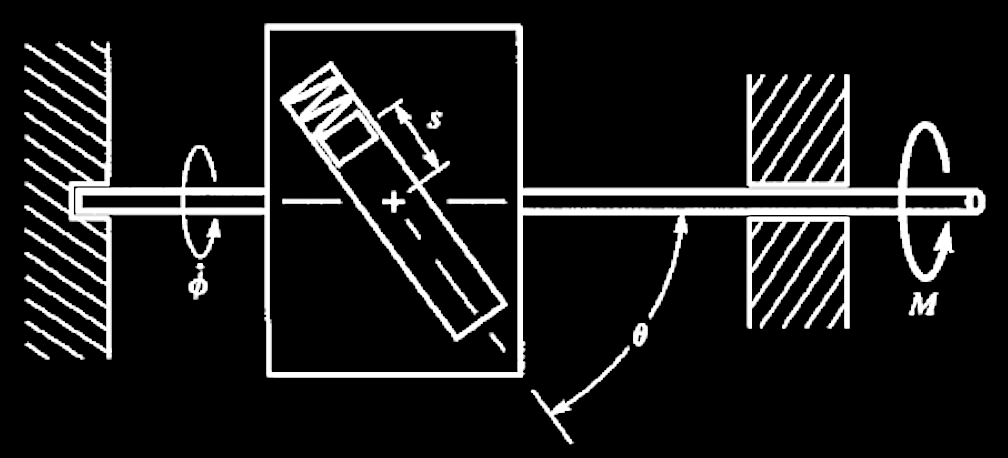
\includegraphics[scale=0.5,frame]{images/Problem_1.png}
\end{figure}

The following coordinate frame will be used to solve this problem:

\begin{figure}[H]
    \centering
    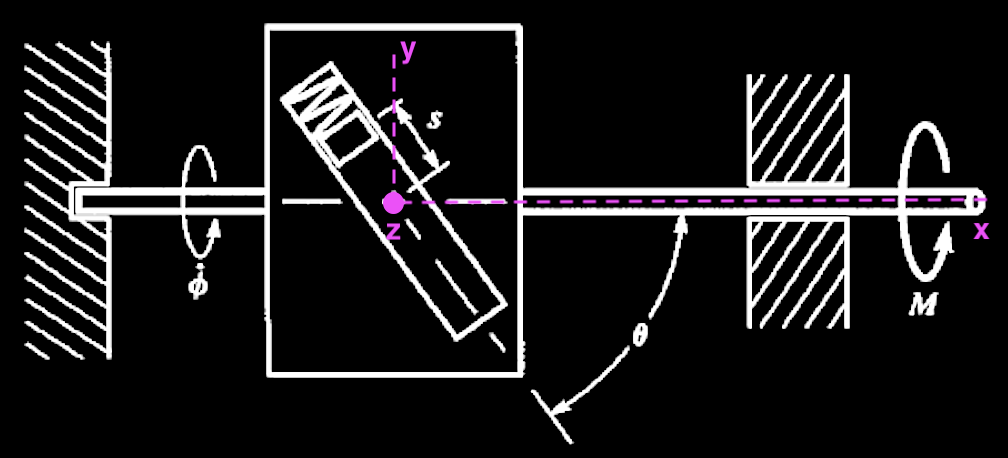
\includegraphics[scale=0.5,frame]{images/Problem_1_cf.png}
\end{figure}

Based on the above coordinate frame, the position of the mass is defined by:

$$ p_{m_1} = \left(\begin{array}{r} -\cos\left(\theta \right)\,s\\ \cos\left(\phi \right)\,s\,\sin\left(\theta \right)\\ \sin\left(\phi \right)\,s\,\sin\left(\theta \right) \end{array}\right) $$

The velocity of $m_1$ is:

$$ v_{m_1} = \left(\begin{array}{r} -\cos\left(\theta \right)\,\dot{s}\\ \cos\left(\phi \right)\,\sin\left(\theta \right)\,\dot{s}-\sin\left(\phi \right)\,s\,\sin\left(\theta \right)\,\dot{\phi} \\ \sin\left(\phi \right)\,\sin\left(\theta \right)\,\dot{s}+\cos\left(\phi \right)\,s\,\sin\left(\theta \right)\,\dot{\phi}  \end{array}\right) $$

The kinetic energy of the system is:

$$ T = \frac{1}{2} I \dot{\phi}^2 +\frac{1}{2} m v_{m_1}^2 $$

Or:

$$ T = \frac{1}{2}m\,{\left({s}^2 \,{\sin \left(\theta \right)}^2 \,{{\dot{\phi}}}^2 +{{\dot{s}}}^2 \right)}+\frac{1}{2}I\,{{\dot{\phi}}}^2  $$

The potential energy is:

$$ V = \frac{1}{2} k s^2 + m g\,s\,\sin(\theta)\cos(\phi)$$

So the Lagrangian is:

$$ L = \frac{1}{2}m\,{\left({s}^2 \,{\sin \left(\theta \right)}^2 \,{{\dot{\phi}}}^2 +{{\dot{s}}}^2 \right)}+\frac{1}{2}I\,{{\dot{\phi}}}^2  - \frac{1}{2} k s^2 - m g\,s\,\sin(\theta)\cos(\phi) $$

Solving for the equations of motion along the generalized coordinate, $s$:

$$ \frac{d}{d t} \frac{\partial L}{\partial \dot{s}} - \frac{\partial L}{\partial s} = 0 $$

The component parts of this equation are:

$$ \frac{\partial L}{\partial s} = 
m\,s\,{\sin \left(\theta \right)}^2 \,{{\left(\dot{\phi} \right)}}^2 -m\,g\,\cos \left(\phi \right)\,\sin \left(\theta \right)-k\,s $$

$$ \frac{\partial L}{\partial \dot{s}}  =
m\,\dot{s} $$

$$ \frac{d}{d t} \frac{\partial L}{\partial \dot{s}} =
m\,\ddot{s} $$

This results in the equation of motion:

$$ m\,\ddot{s}-m\,s\,{\sin \left(\theta \right)}^2 \,{{\dot{\phi}}}^2 +m\,g\,\cos \left(\phi \right)\,\sin \left(\theta \right)+k\,s  = 0 $$

Solving for the equations of motion along the generalized coordinate, $\phi$:

$$ \frac{d}{d t} \frac{\partial L}{\partial \dot{\phi}} - \frac{\partial L}{\partial \phi} = 
\sum_i M_i \frac{\partial \omega_i}{\partial \dot{\phi}} = M $$

The component parts of this equation are:

$$ \frac{\partial L}{\partial \phi} = 
m\,g\,\sin \left(\phi \right)\,s\,\sin \left(\theta \right) $$

$$ \frac{\partial L}{\partial \dot{\phi}}  =
m\,{s}^2 \,{\sin \left(\theta \right)}^2 \,\dot{\phi} +I\,\dot{\phi}  $$

$$ \frac{d}{d t} \frac{\partial L}{\partial \dot{\phi}} =
I\,\ddot{\phi} +m\,{s}^2 \,{\sin \left(\theta \right)}^2 \,\ddot{\phi} +2\,m\,s\,{\sin \left(\theta \right)}^2 \,\dot{s}\,\dot{\phi}  $$

This results in the equation of motion:

$$ I\,\ddot{\phi} +m\,{s}^2 \,{\sin \left(\theta \right)}^2 \,\ddot{\phi}+2\,m\,s\,{\sin \left(\theta \right)}^2 \,\dot{s}\,\dot{\phi}-m\,g\,\sin \left(\phi \right)\,s\,\sin \left(\theta \right) = M $$

The equations of motion for the system are:
\begin{answer}
\begin{equation*}
    \begin{aligned}
        m\,\ddot{s}-m\,s\,{\sin \left(\theta \right)}^2 \,{{\dot{\phi}}}^2 +m\,g\,\cos \left(\phi \right)\,\sin \left(\theta \right)+k\,s  &= 0 \\
        I\,\ddot{\phi} +m\,{s}^2 \,{\sin \left(\theta \right)}^2 \,\ddot{\phi}+2\,m\,s\,{\sin \left(\theta \right)}^2 \,\dot{s}\,\dot{\phi}-m\,g\,\sin \left(\phi \right)\,s\,\sin \left(\theta \right) &= M 
    \end{aligned}
\end{equation*}
\end{answer}

The following MATLAB function was used to solve this problem:

% \color{white}
\hspace*{6em}\inputminted[frame=leftline,fontsize=\footnotesize,lastline=32]{matlab}
{./matlab/Problem_1.m}
% \color{black} 


\subsection*{Problem 2: Nonholonomic System}
\subsubsection*{A known couple $\bm{M(t)}$ is applied to the upper bar.
Force $\bm{F}$, which is applied perpendicularly to the lower bar,
acts to make the velocity of end $\bm{C}$ always be parallel to the line from joint $\bm{A}$ to end $\bm{B}$.
The bars have equal mass $\bm{m}$,
and the system lies in the vertical plane.
Use the method of Lagrange multipliers to derive the equations of motion.}

\begin{figure}[H]
    \centering
    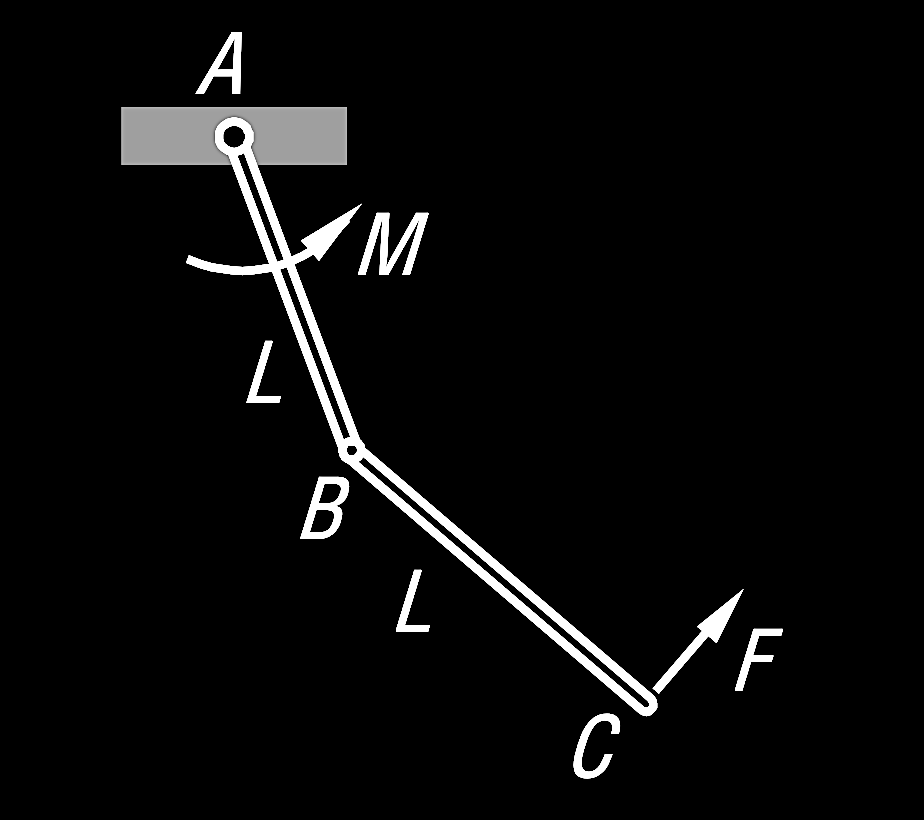
\includegraphics[scale=0.35,frame]{images/Problem_2.png}
\end{figure}

The following coordinate frame will be used to solve this problem:

\begin{figure}[H]
    \centering
    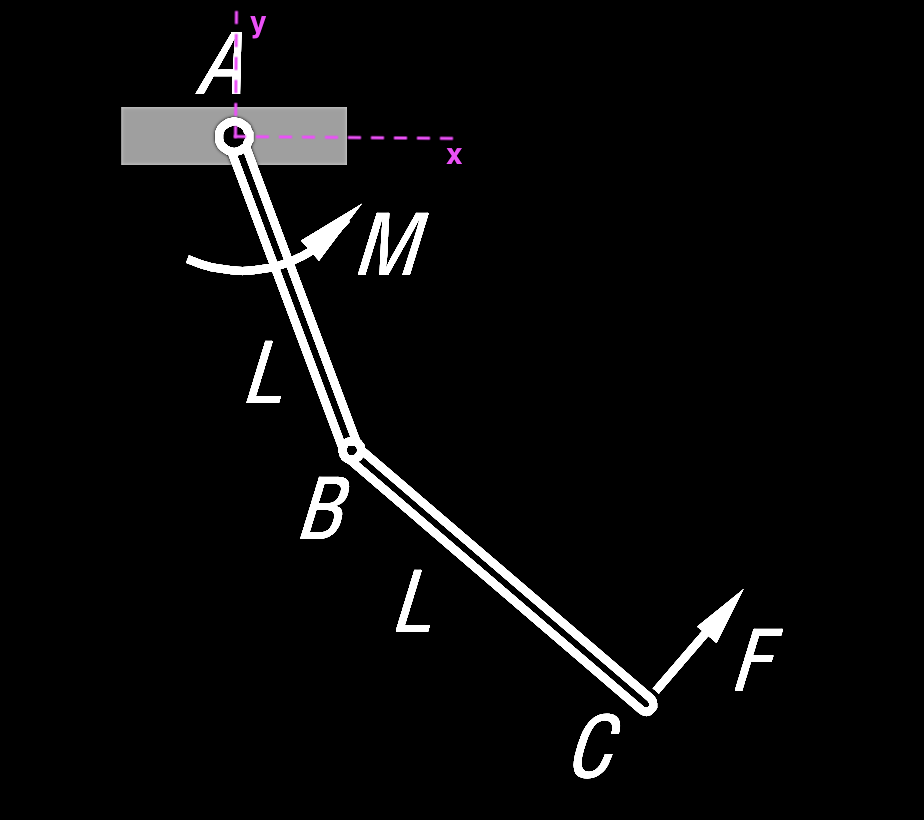
\includegraphics[scale=0.35,frame]{images/Problem_2_cf.png}
\end{figure}

We will define the following positions:

\begin{equation*}
    \begin{aligned}
        p_{\text{cg}_1} &= \left[\begin{array}{c}
            \frac{1}{2}L\,\sin \left(1\theta_1 \right)\\
            \frac{1}{2}L\,\cos \left(\theta_1 \right)
            \end{array}\right]\\
        p_b &= \left[\begin{array}{c}
            L\,\sin \left(\theta_1 \right)\\
            L\,\cos \left(\theta_1 \right)
            \end{array}\right] \\
        p_{\text{cg}_2} &= \left[\begin{array}{c}
            L\,\sin \left(\theta_1 \right)+\frac{1}{2}L\,\sin \left(\theta_2 \right)\\
            L\,\cos \left(\theta_1 \right)+\frac{1}{2}L\,\cos \left(\theta_2 \right)
            \end{array}\right]\\
        p_c &= \left[\begin{array}{c}
            L\,\sin \left(\theta_1 \right)+L\,\sin \left(\theta_2 \right)\\
            L\,\cos \left(\theta_1 \right)+L\,\cos \left(\theta_2 \right)
            \end{array}\right]
    \end{aligned}
\end{equation*}

Taking their derivatives, we get the following velocities:

\begin{equation*}
    \begin{aligned}
        v_{\text{cg}_1} &= \left[\begin{array}{c}
            \frac{1}{2}L\,\cos \left(\theta_1 \right)\,\dot{\theta_1}\\
            -\frac{1}{2}L\,\sin \left(\theta_1 \right)\,\dot{\theta_1}
            \end{array}\right]\\
        v_b &= \left[\begin{array}{c}
            L\,\cos \left(\theta_1 \right)\,\dot{\theta_1} \\
            -L\,\sin \left(\theta_1 \right)\,\dot{\theta_1} 
            \end{array}\right] \\
        v_{\text{cg}_2} &= \left[\begin{array}{c}
            L\,\cos \left(\theta_1 \right)\,\dot{\theta_1} +\frac{1}{2}L\,\cos \left(\theta_2 \right)\,\dot{\theta_2}\\
            -L\,\sin \left(\theta_1 \right)\,\dot{\theta_1} -\frac{1}{2}L\,\sin \left(\theta_2 \right)\,\dot{\theta_2}
            \end{array}\right]\\
        v_c &= \left[\begin{array}{c}
            L\,\cos \left(\theta_1 \right)\,\dot{\theta_1} +L\,\cos \left(\theta_2 \right)\,\dot{\theta_2} \\
            -L\,\sin \left(\theta_1 \right)\,\dot{\theta_1} -L\,\sin \left(\theta_2 \right)\,\dot{\theta_2} 
            \end{array}\right]
    \end{aligned}
\end{equation*}

The constraint, which can be mathematically described as
$ v_c \times r_{B/A} = 0 $, where $r_{B/A} = p_b$ evaluates to:

$$ L^2 \,\dot{\theta_1} +L^2 \,\cos \left(\theta_1 -\theta_2 \right)\,\dot{\theta_2} = 0  $$

Or more simply:

$$ \dot{\theta_1} + \cos \left(\theta_1 -\theta_2 \right)\,\dot{\theta_2} = 0  $$

Putting this in the form of the constraint equation:

$$ \sum_{j=1}^N a_{ij} \dot{q}_j + b_i =
a_{11} \dot{q}_1 + a_{12} \dot{q}_2 + b_1 = 0  $$

We see that:

\begin{equation*}
    \begin{aligned}
        a_{11} &= 1 \\
        a_{12} &= \cos \left(\theta_1 -\theta_2 \right)
    \end{aligned}
\end{equation*}


The centriodal inertia properties of both bars are:

$$ I = I_1  = I_2 = \frac{1}{12} m L^2 $$

The kinetic energy of the system is:

$$ T =  \frac{1}{2} m v_{\text{cg}_1}^2 +
    \frac{1}{2}I \dot{\theta_1}^2 +
    \frac{1}{2} m v_{\text{cg}_1}^2 +
    \frac{1}{2} I \dot{\theta_2}^2 $$

This evaluates to:

$$ T = \frac{2}{3}\,L^2 \,m\,{{\dot{\theta_1}}}^2+
\frac{1}{6}L^2 \,m\,{{\dot{\theta_2}}}^2+
\frac{1}{2}L^2 \,m\,\cos \left(\theta_1 -\theta_2 \right)\,\dot{\theta_2} \,\dot{\theta_1}  $$

The potential energy of the system is:

$$ V = -m\,g\,{\left(L\,\cos \left(\theta_1 \right)+\frac{1}{2}L\,\cos \left(\theta_2 \right)\right)}-\frac{1}{2}m\,g\,L\cos \left(\theta_1 \right) $$

The system Lagrangian is:

\begin{equation*}
    \begin{aligned}
L &= T - V\\
 &= \frac{2}{3}\,L^2 \,m\,{{\dot{\theta_1}}}^2+
\frac{1}{6}L^2 \,m\,{{\dot{\theta_2}}}^2+
\frac{1}{2}L^2 \,m\,\cos \left(\theta_1 -\theta_2 \right)\,\dot{\theta_2} \,\dot{\theta_1} \\
& \ \ \ \ \ \ \ + m\,g\,{\left(L\,\cos \left(\theta_1 \right)+\frac{1}{2}L\,\cos \left(\theta_2 \right)\right)}+\frac{1}{2}m\,g\,L\cos \left(\theta_1 \right)
\end{aligned}
\end{equation*}

Solving for the equations of motion along the generalized coordinate, $\theta_1$:

$$ \frac{d}{d t} \frac{\partial L}{\partial \dot{\theta_1}} - \frac{\partial L}{\partial \theta_1} = 
Q_{\theta_1} + a_{11} \lambda_1 $$

The component parts of this equation are:


$$ \frac{\partial L}{\partial \theta_1} = 
\frac{1}{2}L^2 \,m\,\sin \left(\theta_2 -\theta_1 \right)\,\dot{\theta_2} \,\dot{\theta_1}-
\frac{3}{2}\,L\,g\,m\,\sin \left(\theta_1 \right) $$

$$ \frac{\partial L}{\partial \dot{\theta_1}}  =
\frac{4}{3}\,L^2 \,m\,\dot{\theta_1} +
\frac{1}{2}L^2 \,m\,\cos \left(\theta_1 -\theta_2 \right)\,\dot{\theta_2}  $$

$$ \frac{d}{d t} \frac{\partial L}{\partial \dot{\theta_1}} =
\frac{4}{3}\,L^2 \,m\,\ddot{\theta_1}+
\frac{1}{2}L^2 \,m\,\cos \left(\theta_1 -\theta_2 \right)\,\ddot{\theta_2} -
\frac{1}{2}L^2 \,m\,\sin \left(\theta_1 -\theta_2 \right)\,{\left(\dot{\theta_1} -\dot{\theta_2} \right)}\,\dot{\theta_2} $$


This results in the equation of motion,
where $Q_{\theta_1} = \sum_{i} M \frac{\partial \omega_i}{\partial \dot{\theta_1}} = M $ :

$$ \frac{4}{3}\,L^2 \,m\,\ddot{\theta_1} +
\frac{1}{2}L^2 \,m\,\sin \left(\theta_1 -\theta_2 \right)\,{\dot{\theta_2}}^2+
\frac{1}{2}L^2 \,m\,\cos \left(\theta_1 -\theta_2 \right)\,\ddot{\theta_2}+
\frac{3}{2}\,L\,g\,m\,\sin \left(\theta_1 \right) =
M + \lambda_1 $$

Solving for the equations of motion along the generalized coordinate, $\theta_2$:

$$ \frac{d}{d t} \frac{\partial L}{\partial \dot{\theta_2}} - \frac{\partial L}{\partial \theta_2} = 
Q_{\theta_2} + a_{12} \lambda_1 $$

The component parts of this equation are:

$$ \frac{\partial L}{\partial \theta_2} = 
\frac{1}{2}L^2 \,m\,\sin \left(\theta_2 -\theta_1 \right)\,\dot{\theta_2} \,\dot{\theta_1} -
\frac{3}{2}\,L\,g\,m\,\sin \left(\theta_1 \right) $$

$$ \frac{\partial L}{\partial \dot{\theta_2}}  =
\frac{1}{3}L^2 \,m\,\dot{\theta_2} +
\frac{1}{2}L^2 \,m\,\cos \left(\theta_1 -\theta_2 \right)\,\dot{\theta_1} $$

$$ \frac{d}{d t} \frac{\partial L}{\partial \dot{\theta_2}} =
\frac{1}{3}L^2 \,m\,\ddot{\theta_2} +
\frac{1}{2}L^2 \,m\,\cos \left(\theta_1 -\theta_2 \right)\,\ddot{\theta_1} -
\frac{1}{2}L^2 \,m\,\sin \left(\theta_1 -\theta_2 \right)\,{\left(\dot{\theta_1} -\dot{\theta_2} \right)}\,\dot{\theta_1}  $$

This results in the equation of motion,
where $Q_{\theta_2} = 0 $ :


$$ \frac{1}{3}L^2 \,m\,\ddot{\theta_2}-
\frac{1}{2}L^2 \,m\,\sin \left(\theta_1 -\theta_2 \right)\,{\dot{\theta_1}}^2 +
\frac{1}{2}L^2 \,m\,\cos \left(\theta_1 -\theta_2 \right)\,\ddot{\theta_1}+
\frac{1}{2}L\,g\,m\,\sin \left(\theta_2 \right) =
\cos \left(\theta_1 -\theta_2 \right) \lambda_1$$

The equations of motion for the system are:
\begin{answer}
\begin{equation*}
    \begin{aligned}
        \frac{4}{3}\,L^2 \,m\,\ddot{\theta_1} +
\frac{1}{2}L^2 \,m\,\sin \left(\theta_1 -\theta_2 \right)\,{\dot{\theta_2}}^2+
\frac{1}{2}L^2 \,m\,\cos \left(\theta_1 -\theta_2 \right)\,\ddot{\theta_2}&+
\frac{3}{2}\,L\,g\,m\,\sin \left(\theta_1 \right)\\ &=
M + \lambda_1 \\
\frac{1}{3}L^2 \,m\,\ddot{\theta_2}-
\frac{1}{2}L^2 \,m\,\sin \left(\theta_1 -\theta_2 \right)\,{\dot{\theta_1}}^2 +
\frac{1}{2}L^2 \,m\,\cos \left(\theta_1 -\theta_2 \right)\,\ddot{\theta_1}&+
\frac{1}{2}L\,g\,m\,\sin \left(\theta_2 \right)\\ &=
\cos \left(\theta_1 -\theta_2 \right) \lambda_1
    \end{aligned}
\end{equation*}
\end{answer}

% \color{white}
\hspace*{6em}\inputminted[frame=leftline,fontsize=\footnotesize,lastline=51]{matlab}
{./matlab/Problem_2.m}
% \color{black} 

% % \color{white}
% \hspace*{6em}\inputminted[frame=leftline,fontsize=\footnotesize]{matlab}
% {./matlab/Q6_8.m}
% % \color{black} 

% \begin{figure}[H]
%     \centering
%     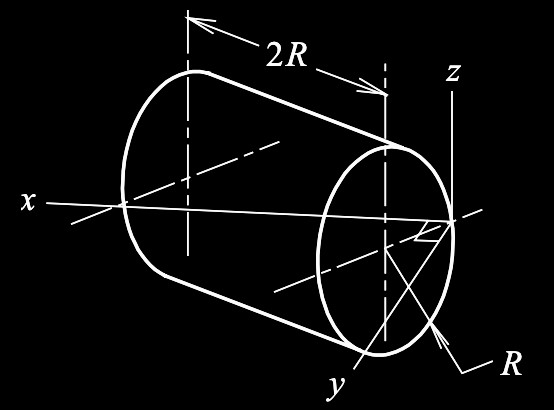
\includegraphics[scale=0.7,frame]{images/Q5_13.png}
% \end{figure}




\end{document}

